\begin{frame}
\frametitle{quiz Q1}
\begin{minipage}{3cm}
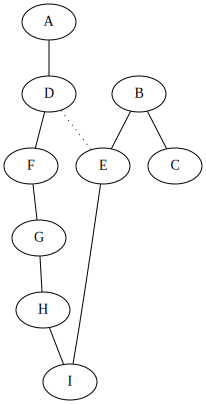
\includegraphics[width=2.9cm]{quiz-graph}
\end{minipage}
\begin{minipage}{10cm}
\begin{itemize}\small
    \item wrong \textit{next hops} (not distances) in best case:
        \begin{itemize} \small
        \item \{E,I\}$\rightarrow$\{A,D,F\}
        \item \{D,F\}$\rightarrow$\{E,I,B,C\}
        \end{itemize}
    \item best case: G/H already has chosen `best' next hop for A/D/E/B/C
    \item E, D will realize next hops are wrong immediately, but need to get correct
        next hops to each other, best case:
        \begin{itemize} \small
            \item E$\rightarrow$I$\rightarrow$H to update I + H's distance to D/A/F to $\infty$ (2 updates)
            \item G$\rightarrow$H$\rightarrow$I$\rightarrow$E to update H+ I + E's next hop to D/A/F (3 updates)
            \item plus same 3 updates for D+F+G's next hops to E/B/C
        \end{itemize}
    \item 10 updates?
\end{itemize}
\end{minipage}
\end{frame}

\begin{frame}
\frametitle{quiz Q3}
    \begin{itemize}
        \item should not have had Q as customer + peer of M
    \end{itemize}
\end{frame}

\begin{frame}
    \frametitle{quiz Q4}
    \begin{itemize}
        \item next hop = which router IP to go to next
            \begin{itemize}
                \item different for connections to different part of other network
            \end{itemize}
        \item AS path = which ASs route went through
            \begin{itemize}
                \item add AS to AS path no matter how long it goes through AS
                \item technically could prefix route from one announcement more times, but rare choice
                \item MED is how we express our preferences about which way through AS to use
            \end{itemize}
        \item how specific
            \begin{itemize}
                \item generally not going to change original announcement
            \end{itemize}
    \end{itemize}
\end{frame}
